\documentclass[11pt,letterpaper]{article}
\usepackage[spanish,es-tabla]{babel}
\usepackage[utf8]{inputenc}
\usepackage[T1]{fontenc}
\usepackage{lmodern}
\usepackage[margin=2.3cm]{geometry}
\usepackage{graphicx}
\usepackage{booktabs}
\usepackage{tabularx}
\usepackage{array}
\usepackage{xcolor}
\usepackage{colortbl}
\usepackage{enumitem}
\usepackage{float}
\usepackage{listings}
\usepackage{hyperref}

\definecolor{azul}{HTML}{1F3A68}
\definecolor{grisclaro}{HTML}{F3F5F9}
\hypersetup{colorlinks=true, linkcolor=azul, urlcolor=azul}
\newcolumntype{Y}{>{\raggedright\arraybackslash}X}
\renewcommand{\arraystretch}{1.3}

\lstset{
  basicstyle=\ttfamily\footnotesize,
  backgroundcolor=\color{grisclaro},
  frame=single, rulecolor=\color{gray!40},
  breaklines=true, columns=fullflexible,
  keywordstyle=\color{azul}\bfseries,
  commentstyle=\color{gray}\itshape,
  literate={á}{{\'a}}1 {é}{{\'e}}1 {í}{{\'i}}1 {ó}{{\'o}}1 {ú}{{\'u}}1 {ñ}{{\~n}}1
}

\begin{document}

% ================================================================ PORTADA
\begin{titlepage}
  \centering
  {\large Universidad Autónoma de Ciudad Juárez\par}
  {\large Instituto de Ingeniería y Tecnología\par}
  \vspace{2.5cm}
  {\Huge\bfseries\color{azul} Sistema web de gestión académica para cursos\par}
  \vspace{0.8cm}
  {\Large Análisis y priorización de atributos de calidad\par}
  \vspace{3cm}
  {\large Marlene Itzel Muñoz González\par}
  \vspace{0.4cm}
  {\large Ingeniería en Software\par}
  \vfill
  {\large \today\par}
\end{titlepage}

\tableofcontents
\newpage

% ================================================================ 1
\section{Contexto y necesidades del cliente}

El director de una institución educativa solicita una página web en la que los
estudiantes consulten sus calificaciones, materias e información académica, y en
la que los profesores registren y modifiquen calificaciones mediante usuario y
contraseña. Del planteamiento se extraen las siguientes necesidades:

\begin{itemize}[leftmargin=*]
  \item \textbf{Protección de la información:} nadie sin autorización debe ver las
        calificaciones.
  \item \textbf{Rapidez y facilidad de uso} para estudiantes y profesores.
  \item \textbf{Disponibilidad} en los momentos en que los estudiantes consultan
        sus resultados.
  \item \textbf{Restricciones:} presupuesto limitado y poco tiempo de desarrollo.
\end{itemize}

% ================================================================ 2
\section{Identificación de cinco atributos de calidad}

\begin{table}[H]
\centering
\begin{tabularx}{\textwidth}{>{\bfseries}l Y Y}
\toprule
\rowcolor{grisclaro}
Atributo & Definición & Necesidad del cliente que lo origina \\
\midrule
Seguridad & Capacidad del sistema para proteger la información y permitir el acceso
solo a usuarios autorizados según su rol. &
``Me preocupa que cualquier persona pueda acceder a las calificaciones''; acceso de
profesores con usuario y contraseña. \\
Usabilidad & Facilidad con la que los usuarios aprenden a usar el sistema y realizan
sus tareas sin errores. & ``Quiero que la página sea fácil de utilizar''. \\
Disponibilidad & Proporción de tiempo en que el sistema está operativo y accesible. &
``Que esté disponible cuando los estudiantes necesiten consultar sus resultados''. \\
Rendimiento & Tiempo de respuesta y capacidad de atender solicitudes. &
``Quiero que la página sea rápida''. \\
Mantenibilidad & Facilidad para modificar, corregir y ampliar el sistema con bajo
costo. & Presupuesto limitado y entrega en poco tiempo. \\
\bottomrule
\end{tabularx}
\caption{Atributos de calidad identificados.}
\end{table}

% ================================================================ 3
\section{Selección y prioridad de los tres atributos principales}

\begin{enumerate}[leftmargin=*]
  \item \textbf{Seguridad} (prioridad 1)
  \item \textbf{Usabilidad} (prioridad 2)
  \item \textbf{Disponibilidad} (prioridad 3)
\end{enumerate}

Rendimiento y mantenibilidad no se descartan: el rendimiento se obtiene de forma
natural con una aplicación ligera y pocos usuarios, y la mantenibilidad se atiende
eligiendo tecnologías simples (Flask y SQLite). Sin embargo, por el presupuesto y el
tiempo limitados, el esfuerzo se concentra en los tres atributos anteriores.

% ================================================================ 4
\section{Tabla comparativa y justificación}

\begin{table}[H]
\centering
\small
\begin{tabularx}{\textwidth}{c >{\bfseries}l c c Y}
\toprule
\rowcolor{grisclaro}
Prioridad & Atributo & Impacto & Costo & Justificación \\
\midrule
1 & Seguridad & Alto & Bajo &
Las calificaciones son datos personales; una filtración o una modificación indebida
dañaría la confianza en la institución y podría tener consecuencias legales. Es la
única preocupación que el cliente expresa como temor explícito. Además, en Flask se
logra con bajo costo (hash de contraseñas, sesiones y control por rol). \\
2 & Usabilidad & Alto & Bajo &
Los usuarios no son técnicos y deben usar el sistema sin capacitación; si es
confuso, los profesores cometerán errores al capturar y los estudiantes saturarán
la dirección con preguntas. Con HTML y CSS simples se logra sin costo extra. \\
3 & Disponibilidad & Medio-alto & Medio &
La consulta se concentra en fechas de cierre de periodo; si el sistema cae en ese
momento pierde su valor. Se prioriza por debajo de la seguridad porque una caída
breve es recuperable, mientras que una filtración no lo es. \\
\midrule
4 & Rendimiento & Medio & Bajo &
Con pocos usuarios y consultas sencillas el tiempo de respuesta ya es bajo; no
requiere inversión adicional. \\
5 & Mantenibilidad & Medio & Bajo &
Importante a futuro, pero el cliente no la pide directamente; se cubre con código
organizado y documentado. \\
\bottomrule
\end{tabularx}
\caption{Tabla comparativa de atributos de calidad.}
\end{table}

% ================================================================ 5
\section{Conflictos entre atributos de calidad}

\subsection{Conflicto 1: Seguridad vs.\ Usabilidad}

Las medidas de seguridad agregan pasos al usuario: iniciar sesión, cierre de sesión
por inactividad y bloqueo tras varios intentos fallidos. Si son demasiado estrictas,
el sistema se vuelve molesto (por ejemplo, contraseñas muy complejas o sesiones que
expiran cada pocos minutos).

\textbf{Resolución:}
\begin{itemize}[leftmargin=*]
  \item La sesión expira a los 30 minutos: suficiente para capturar calificaciones
        sin interrupciones, pero sin dejar sesiones abiertas indefinidamente.
  \item El bloqueo ocurre solo tras 5 intentos fallidos y dura 5 minutos, con un
        mensaje claro que indica cuánto esperar.
  \item Después de iniciar sesión, el sistema lleva a cada usuario directamente a su
        panel según su rol, reduciendo pasos.
  \item El mensaje de error es claro pero genérico (``Usuario o contraseña
        incorrectos''), para no revelar qué usuarios existen.
\end{itemize}

\subsection{Conflicto 2: Disponibilidad vs.\ Costo y tiempo de desarrollo}

Una alta disponibilidad real requiere servidores redundantes, balanceo de carga y
réplicas de base de datos, lo que choca con el presupuesto limitado y con la entrega
en poco tiempo.

\textbf{Resolución:}
\begin{itemize}[leftmargin=*]
  \item Se usa SQLite, una base de datos embebida que no depende de un servidor
        externo (un punto de falla menos y sin costo de licencias).
  \item Se agregó la ruta \texttt{/salud} para que un servicio de monitoreo gratuito
        avise si el sistema deja de responder.
  \item Los errores se manejan con páginas amigables en lugar de caídas del servidor.
  \item Se recomienda desplegar en un servicio de hospedaje económico con reinicio
        automático y respaldar el archivo de la base de datos diariamente; la
        redundancia se deja como mejora futura cuando haya presupuesto.
\end{itemize}

% ================================================================ 6
\section{Diseño y desarrollo del sistema}

\subsection{Tecnologías}
\begin{itemize}[leftmargin=*]
  \item \textbf{Back-end:} Python 3 con Flask.
  \item \textbf{Front-end:} plantillas HTML (Jinja2) y una hoja de estilos CSS propia.
  \item \textbf{Base de datos:} SQLite con tres tablas: \texttt{usuarios},
        \texttt{materias} e \texttt{inscripciones}.
\end{itemize}

\subsection{Funcionalidades}
\begin{itemize}[leftmargin=*]
  \item Inicio de sesión para estudiantes y profesores.
  \item Panel del estudiante: materias, profesor, calificación y promedio general.
  \item Panel del profesor: lista de sus materias y formulario para registrar o
        modificar calificaciones (0 a 100, o pendiente).
  \item Cierre de sesión.
\end{itemize}

\subsection{Prototipo}

\begin{figure}[H]
  \centering
  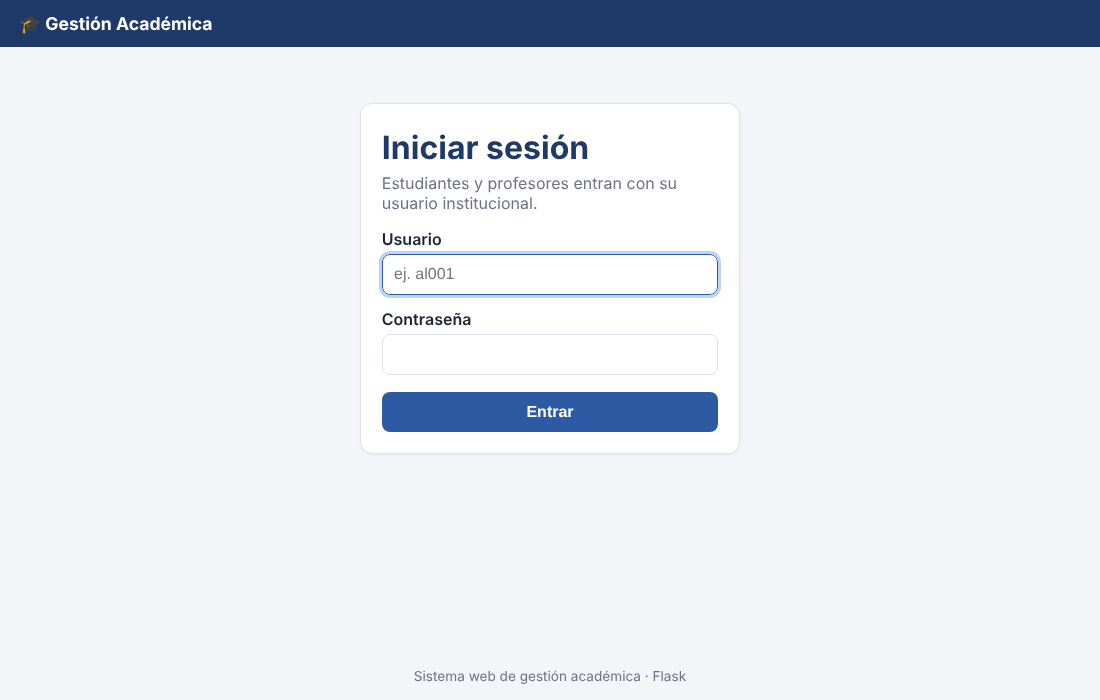
\includegraphics[width=0.75\textwidth]{capturas/01_login.png}
  \caption{Pantalla de inicio de sesión.}
\end{figure}

\begin{figure}[H]
  \centering
  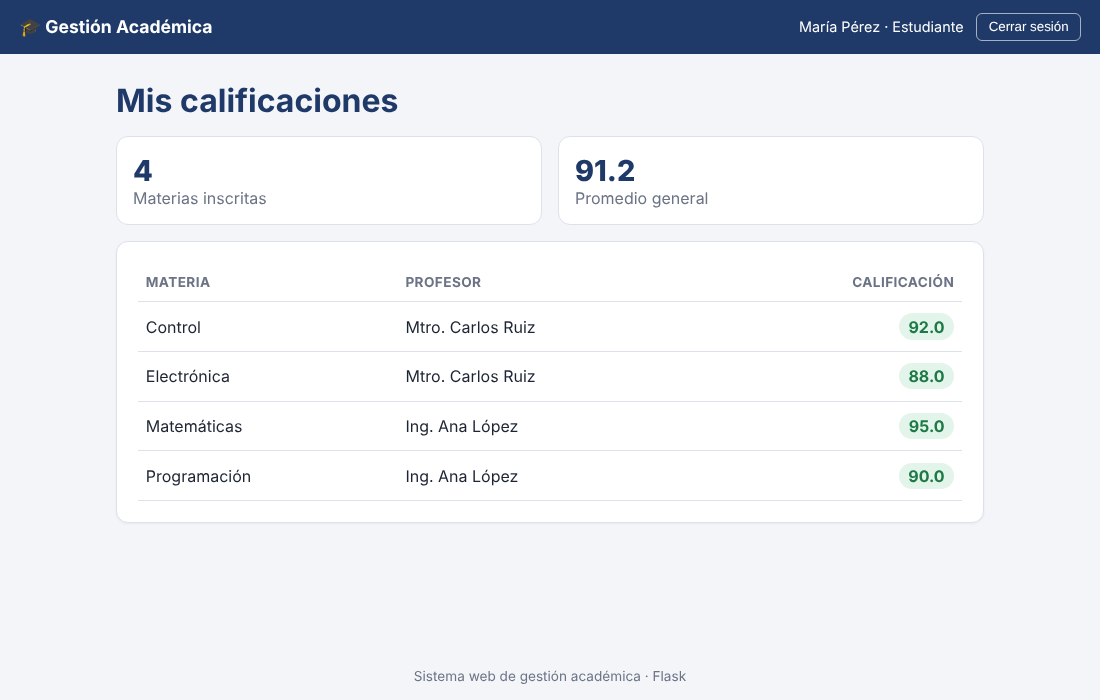
\includegraphics[width=0.75\textwidth]{capturas/03_estudiante.png}
  \caption{Panel del estudiante con sus calificaciones y promedio.}
\end{figure}

\begin{figure}[H]
  \centering
  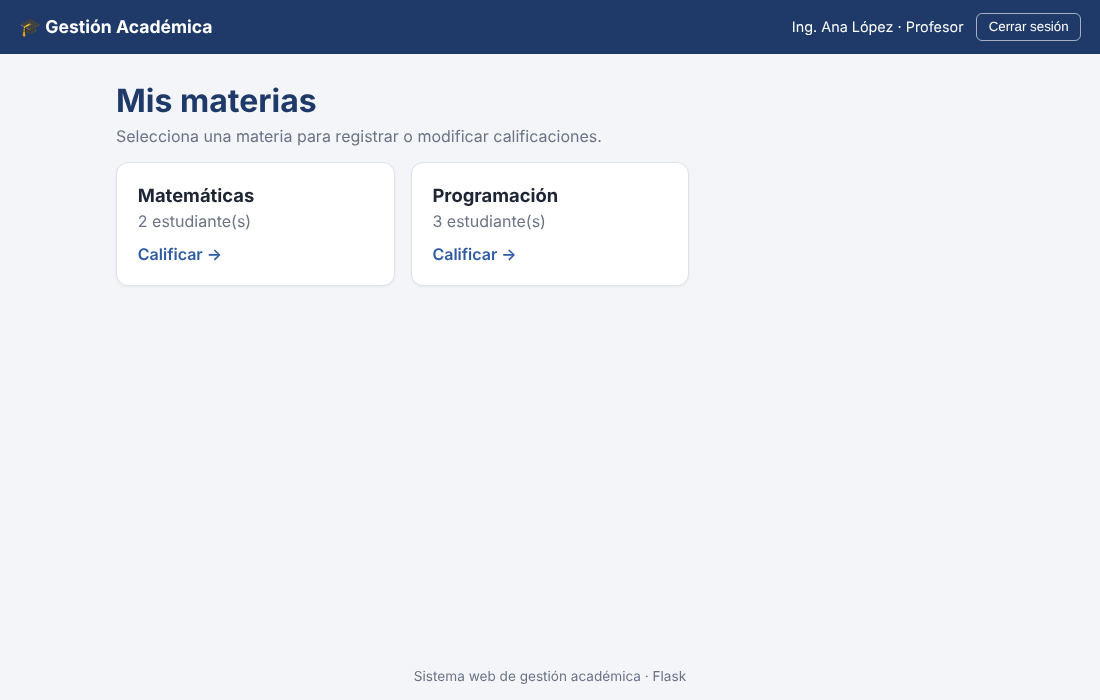
\includegraphics[width=0.75\textwidth]{capturas/05_profesor.png}
  \caption{Panel del profesor con sus materias.}
\end{figure}

\begin{figure}[H]
  \centering
  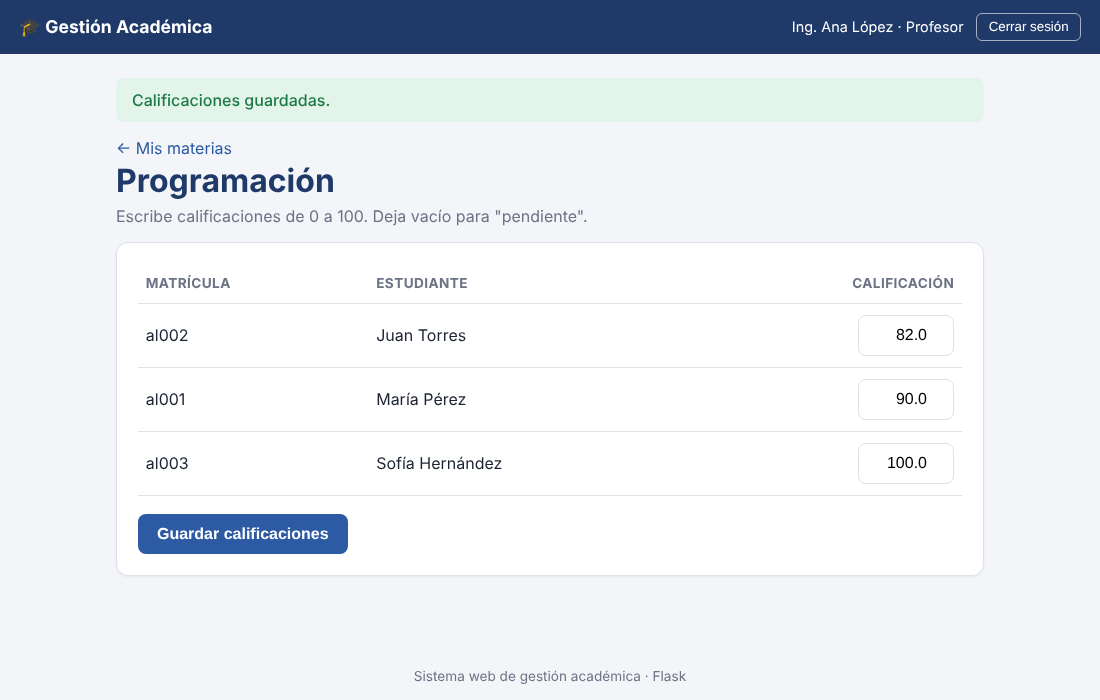
\includegraphics[width=0.75\textwidth]{capturas/06_calificar.png}
  \caption{Registro y modificación de calificaciones.}
\end{figure}

% ================================================================ 7
\section{Aplicación de los atributos de calidad en el sistema}

\subsection{Seguridad}
\begin{itemize}[leftmargin=*]
  \item \textbf{Contraseñas con hash:} se guardan con \texttt{generate\_password\_hash}
        de Werkzeug (scrypt); nunca en texto plano.
  \item \textbf{Control de acceso por rol:} el decorador \texttt{login\_requerido}
        exige sesión y verifica el rol; un estudiante que intenta entrar al panel del
        profesor recibe un error 403.
  \item \textbf{Aislamiento de datos:} el estudiante solo ve sus calificaciones,
        porque su identificador se toma de la sesión y no de la URL. Un profesor solo
        puede editar las materias que tiene asignadas.
  \item \textbf{Protección CSRF:} todos los formularios llevan un token secreto que
        se valida en cada petición POST.
  \item \textbf{Sesiones seguras:} cookies \texttt{HttpOnly} y \texttt{SameSite=Lax},
        regeneración de sesión al iniciar y expiración a los 30 minutos.
  \item \textbf{Protección contra fuerza bruta:} bloqueo de 5 minutos tras 5 intentos
        fallidos.
  \item \textbf{Consultas parametrizadas} para evitar inyección SQL, validación de
        calificaciones (0 a 100) y cabeceras de seguridad (\texttt{X-Frame-Options},
        \texttt{Content-Security-Policy}, \texttt{Cache-Control: no-store}).
\end{itemize}

\begin{lstlisting}[language=Python, caption={Control de acceso por rol}]
def login_requerido(rol=None):
    def decorador(vista):
        @wraps(vista)
        def envoltura(*args, **kwargs):
            g.usuario = usuario_actual()
            if g.usuario is None:
                return redirect(url_for("login"))
            if rol and g.usuario["rol"] != rol:
                abort(403)
            return vista(*args, **kwargs)
        return envoltura
    return decorador
\end{lstlisting}

\subsection{Usabilidad}
\begin{itemize}[leftmargin=*]
  \item Interfaz limpia con pocas opciones por pantalla y redirección automática al
        panel correspondiente al rol.
  \item Calificaciones con código de color: verde (aprobada), rojo (reprobada) y
        ámbar (pendiente).
  \item Mensajes de confirmación y de error claros (``Calificaciones guardadas'').
  \item Diseño responsivo: funciona en teléfonos celulares, donde los estudiantes
        suelen consultar.
  \item Accesibilidad: etiquetas en todos los campos, foco visible y buen contraste.
\end{itemize}

\begin{figure}[H]
  \centering
  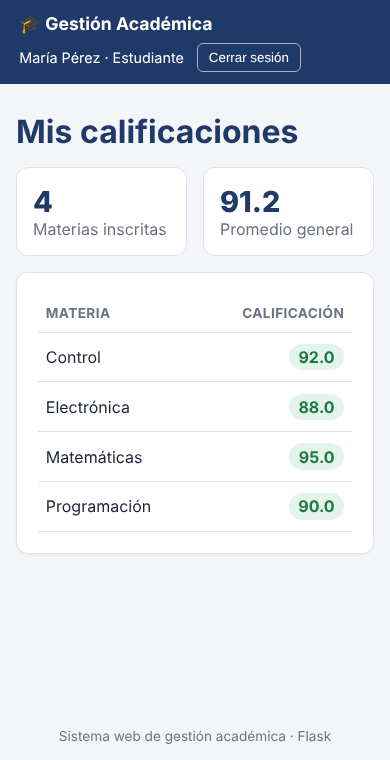
\includegraphics[width=0.3\textwidth]{capturas/07_movil.png}
  \caption{Vista del estudiante en un teléfono celular.}
\end{figure}

\subsection{Disponibilidad}
\begin{itemize}[leftmargin=*]
  \item Base de datos SQLite embebida: sin servidor externo que pueda fallar.
  \item Ruta \texttt{/salud} que verifica la conexión a la base de datos y responde
        200 (``ok'') o 503 (error), útil para monitoreo.
  \item Manejadores de error (400, 403, 404 y 500) que muestran páginas amigables
        en lugar de caídas.
  \item Índices en la tabla \texttt{inscripciones} para mantener respuestas rápidas
        en épocas de alta consulta.
\end{itemize}

% ================================================================ 8
\section{Evidencias de la aplicación de los atributos}

\subsection{Pruebas automatizadas}
Se desarrollaron 15 pruebas con \texttt{unittest} que verifican cada atributo. Todas
se ejecutaron con éxito.

\begin{table}[H]
\centering
\small
\begin{tabularx}{\textwidth}{l Y c}
\toprule
\rowcolor{grisclaro}
Atributo & Prueba & Resultado \\
\midrule
Seguridad & Las contraseñas se almacenan con hash & Aprobada \\
Seguridad & Sin sesión, todas las rutas redirigen al login & Aprobada \\
Seguridad & Login incorrecto devuelve un mensaje genérico (401) & Aprobada \\
Seguridad & Bloqueo tras 5 intentos fallidos (429) & Aprobada \\
Seguridad & Un estudiante no accede al panel del profesor (403) & Aprobada \\
Seguridad & Un estudiante solo ve sus propias calificaciones & Aprobada \\
Seguridad & Un profesor no puede editar una materia ajena (403) & Aprobada \\
Seguridad & Peticiones POST sin token CSRF son rechazadas (400) & Aprobada \\
Seguridad & Cookies HttpOnly/SameSite y cabeceras de seguridad & Aprobada \\
Seguridad & No se guardan calificaciones fuera del rango 0--100 & Aprobada \\
Usabilidad & El profesor registra y el estudiante ve el cambio & Aprobada \\
Usabilidad & Redirección automática según el rol & Aprobada \\
Usabilidad & Página 404 amigable & Aprobada \\
Disponibilidad & La ruta \texttt{/salud} responde ``ok'' & Aprobada \\
Rendimiento & Tiempo promedio de respuesta menor a 200 ms (medido: 1.6 ms) & Aprobada \\
\bottomrule
\end{tabularx}
\caption{Resultados de las pruebas de atributos de calidad.}
\end{table}

\subsection{Evidencias visuales}

\begin{figure}[H]
  \centering
  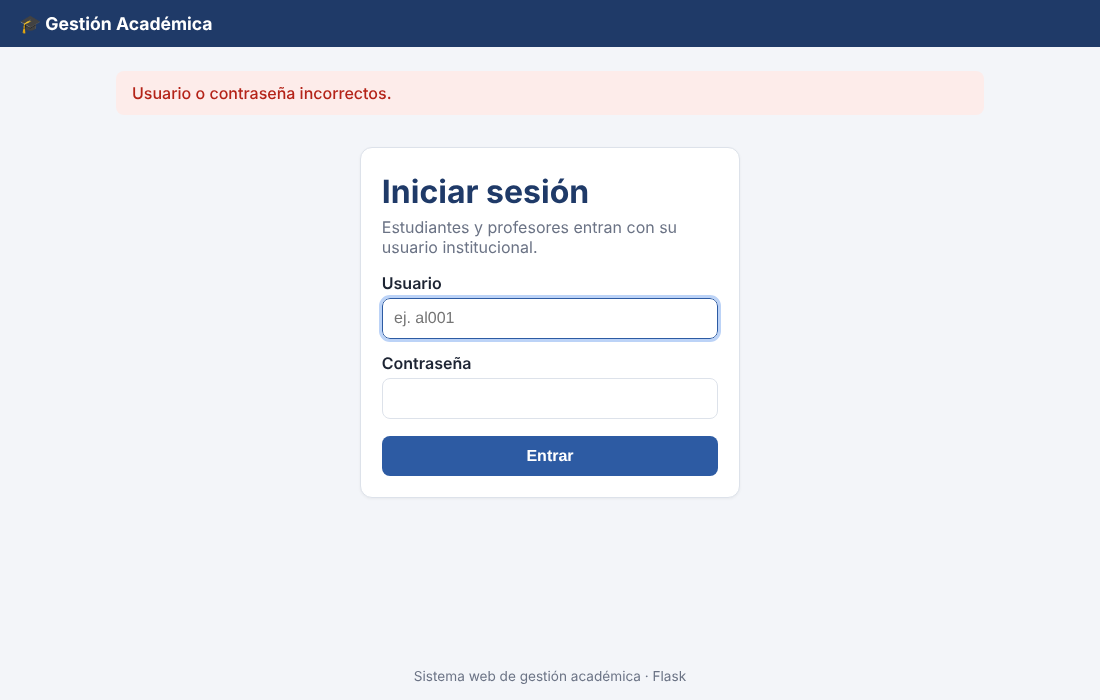
\includegraphics[width=0.7\textwidth]{capturas/02_login_error.png}
  \caption{Seguridad: mensaje genérico ante credenciales incorrectas.}
\end{figure}

\begin{figure}[H]
  \centering
  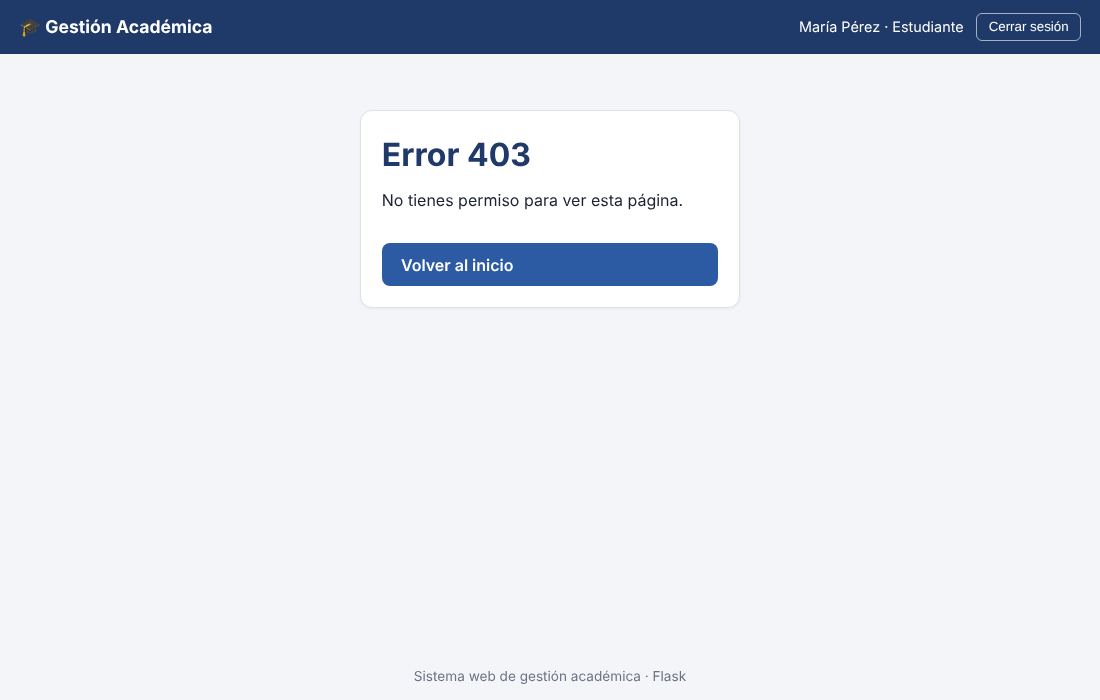
\includegraphics[width=0.7\textwidth]{capturas/04_acceso_denegado.png}
  \caption{Seguridad: un estudiante intenta entrar al panel del profesor y es
  rechazado (403).}
\end{figure}

% ================================================================ 9
\section{Conclusión}

Ante un presupuesto y un tiempo limitados, no es posible maximizar todos los
atributos de calidad a la vez, por lo que es necesario priorizar. Se eligió la
seguridad como prioridad principal porque protege datos personales y responde a la
preocupación más importante del cliente; después, la usabilidad, para que estudiantes
y profesores usen el sistema sin capacitación; y por último, la disponibilidad,
atendida con soluciones de bajo costo. Flask, HTML, CSS y SQLite permitieron cumplir
estos atributos con una solución sencilla, económica y fácil de mantener, y las
pruebas automatizadas demuestran que las decisiones se reflejan en el sistema.

\end{document}
